\documentclass{article}

\usepackage{float}
\usepackage{microtype}
\usepackage{indentfirst}
\usepackage{amsmath}
\usepackage{tikz}
\usepackage{graphicx}
\graphicspath{{figuras/}}
\usetikzlibrary{arrows,automata}
\usepackage[utf8]{inputenc}
\usepackage[portuguese]{babel}

\title{Relatório 3 \- MIPS Multiciclo}
\author{%
    Mikael Luan da Silva Saraiva, \\
    João Vitor Maia Neves Cordeiro, \\
    Paola de Oliveira Abel
    }

\begin{document}
    \maketitle

    \section{Introdução}

    Neste projeto desenvolveremos um PROCESSador MIPS multiciclo, criando seus
    arquivos de descrição em VHDL e realizando as devidas simulações além de
    analisar seu funcionamento.

    \section{Descrição do Sistema}

    Eu preciso completar isso

    \section{Principais características}

    Contem um unidade de memoria, banco de registradores com 32 registradores,
    um a ULA, possui PROCESSamento multiciclo é mais rápido que o monociclo,
    pois pode realizar mais de uma etapa de um PROCESSo por ciclo de clock,
    desde que usem áreas diferentes. No projeto multiciclo consideramos que um
    ciclo de clock pode acomodar no máximo uma das seguintes operações: Um
    acesso a memoria, um acesso ao banco de registradores (duas leituras e uma
    escrita, ou uma operação da ULA). Consequentemente quaisquer dados
    produzidos por uma dessas três unidades funcionais precisam ser salvos em
    um registrador temporário para uso em um ciclo posterior, se eles não forem
    salvos poderia haver a possibilidade de uma disputa de sincronização,
    levando ao uso de um valor incorreto.

        \subsection{Circuitos}


        \begin{figure}[H]
            \centering % para centralizarmos a figura
            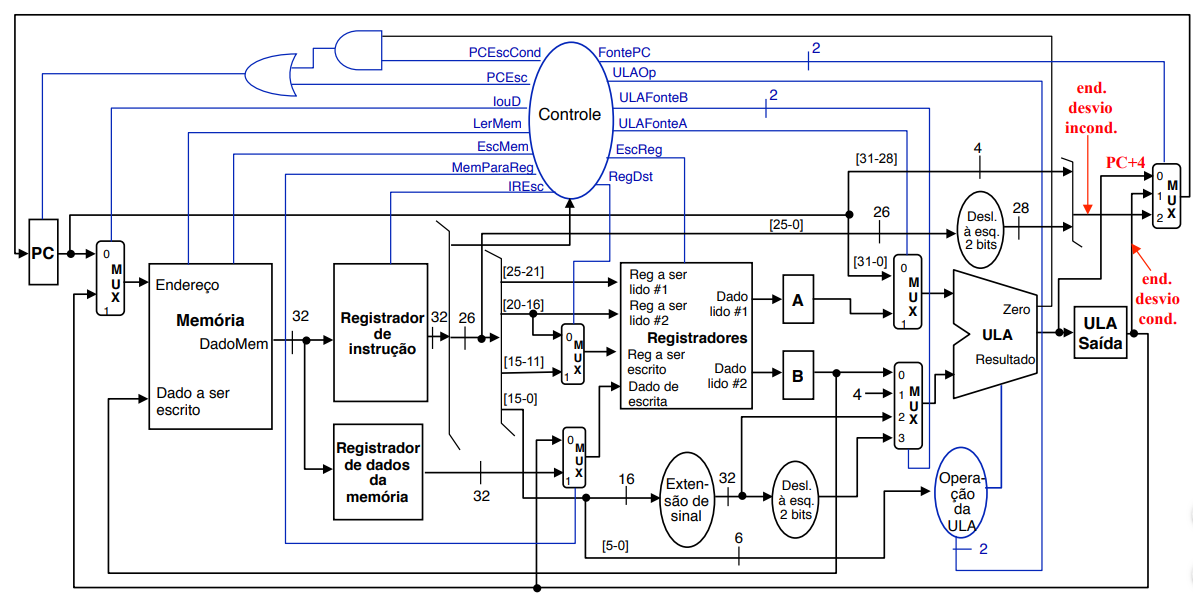
\includegraphics[width=\textwidth]{circuito_mips.png} % leia abaixo
            \caption{Circuito do MIPS multiciclo.}
            \label{figura:mips}
        \end{figure}

        \subsection{Diagramas}

        \subsection{Transição de Estados}

        Pegar nos slides.

        \subsection{Maquinas de Estado}

        \begin{figure}[H]
            \centering
            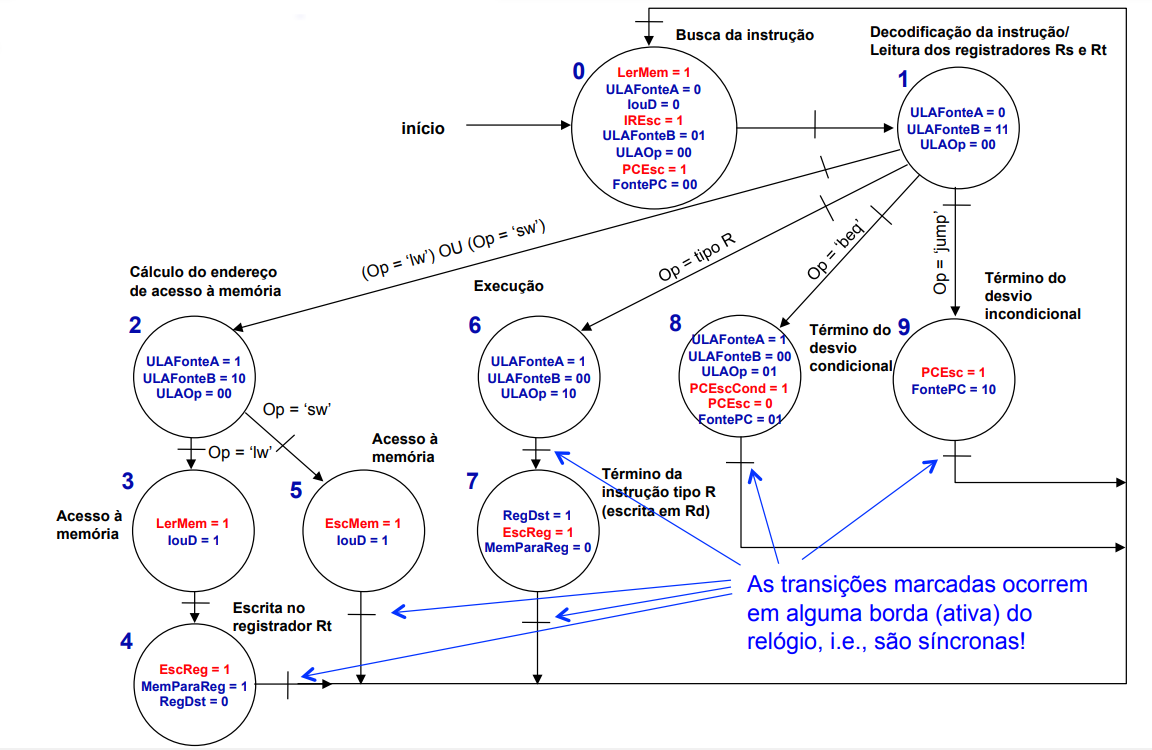
\includegraphics[scale=1.5]{maquina_estados.png}
            \caption{Maquina de estados do MIPS multiciclo.}
            \label{figura:maquina}
        \end{figure}

        \section{Resultados de atrasos}

        A seguir é apresentado os dados adquiridos após a compilação do MIPS
        multiciclo.

        \begin{figure}[H]
            \centering
            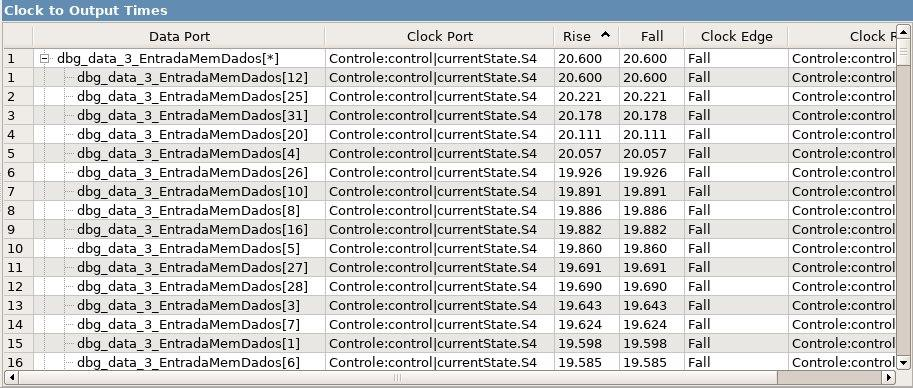
\includegraphics[width=\textwidth]{clock_to_output_times.jpg}
            \caption{Clock to Output Times.}
            \label{figura:mips}
        \end{figure}

        \begin{figure}[H]
            \centering
            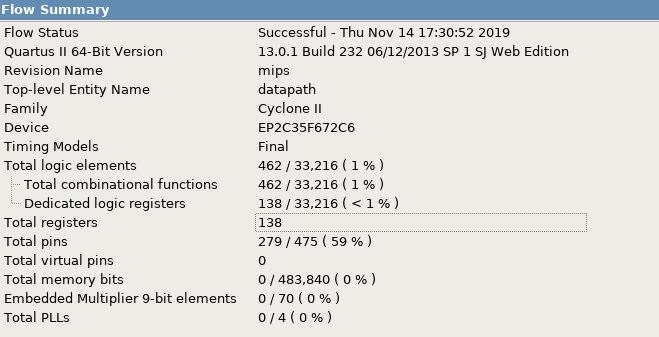
\includegraphics[width=\textwidth]{flow_summary.jpg}
            \caption{Flow Summary.}
            \label{figura:mips}
        \end{figure}

        \begin{figure}[H]
            \centering
            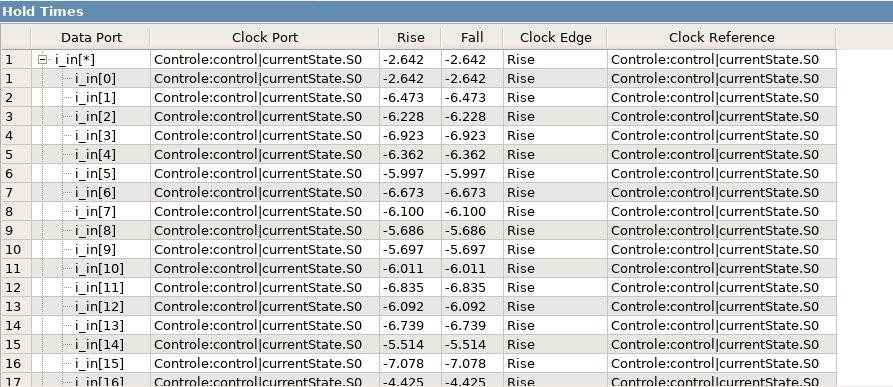
\includegraphics[width=\textwidth]{hold_times.jpg}
            \caption{Hold Times.}
            \label{figura:mips}
        \end{figure}

        \begin{figure}[H]
            \centering
            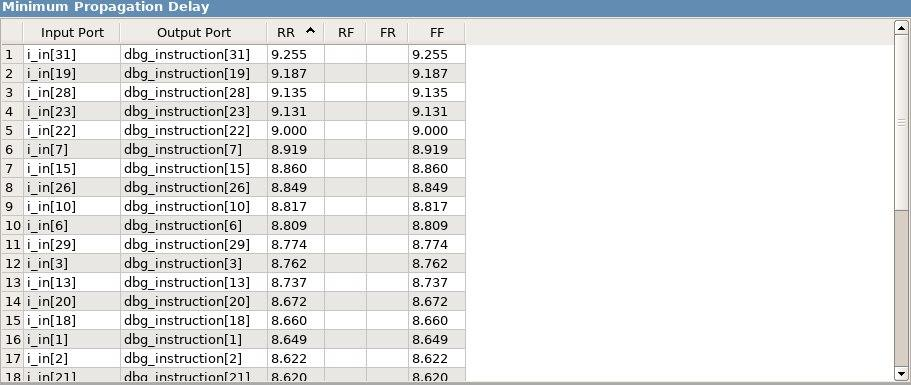
\includegraphics[width=\textwidth]{minimum_propagation_delay.jpg}
            \caption{Minimum Propagation Delay.}
            \label{figura:mips}
        \end{figure}

        \begin{figure}[H]
            \centering
            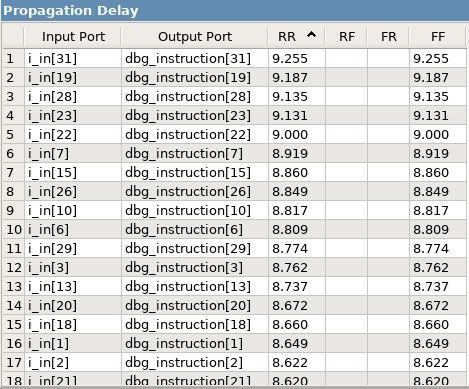
\includegraphics[width=\textwidth]{propagation_delay.jpg}
            \caption{Propagation Delay.}
            \label{figura:mips}
        \end{figure}

        \begin{figure}[H]
            \centering
            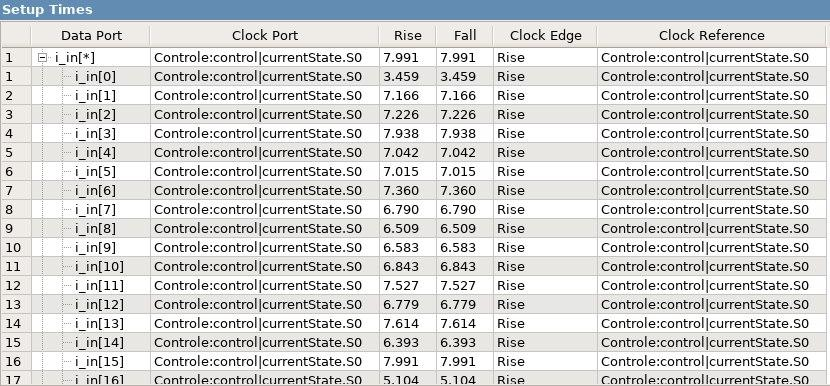
\includegraphics[width=\textwidth]{setup_times.jpg}
            \caption{Setup Times.}
            \label{figura:mips}
        \end{figure}


    \section{Utilização da placa}

    Eu preciso completar isso

    \section{Discussão dos resultados}

    Durante os testes realizados com essa implementação do MIPS, a percepção geral do grupo é que 
    uma implementação de um sistema digital complexo como um processador exige muito mais do que apenas
    a descrição do sistema em VHDL (ou outra linguagem de descrição de hardware). É necessário a aplicação
    de padrões de projeto e metodologias de teste mais ágeis do que o uso de arquivos .do com ModelSim.

    A simulação das instruções implementadas foi a parte mais complicada em questão de complexidade, além
    de não ter ficado muito claro como é feito o uso do Testbench, o software padrão de simulação da
    disciplina (ModelSim Altera) tem pouca documentação online e consome quantidades elevadas de recursos
    de hardware. Quanto maior a simulação, mais hardware consumido, até o ponto onde a simulação não consegue
    continuar, isso limitou significativament o teste de um bloco grande de instruções e nos levou a optar
    por executar isoladamente cada instrução implementada.

    Apesar de ser apenas uma versão resumida do MIPS, a implementação realizada contribui com a fixação
    de conhecimentos adquiridos tanto durante as aulas práticas quanto teóricas.

    \section{Conclusões}

    Eu preciso completar isso

\end{document}
